\documentclass[11pt, letterpaper]{article}

\usepackage[margin=1in]{geometry}
\usepackage[T1]{fontenc}
\usepackage[utf8]{inputenc}
\usepackage{amsmath}
\usepackage{amssymb}
\usepackage{booktabs}
\usepackage{array}
\usepackage{multirow}
\usepackage{hyperref}
\usepackage{setspace}
\usepackage{parskip}
\usepackage{xcolor}
\usepackage{titlesec}
\usepackage{graphicx}
\usepackage{caption}
\usepackage{subcaption}
\usepackage{tikz}
\usepackage{natbib}
\usetikzlibrary{arrows.meta, positioning, fit, backgrounds}

\hypersetup{colorlinks=true, linkcolor=blue, citecolor=blue, urlcolor=blue}
\onehalfspacing

\definecolor{qNavy}{RGB}{15,40,90}
\definecolor{qMid}{RGB}{0,100,180}
\definecolor{qLight}{RGB}{220,232,245}
\definecolor{qGold}{RGB}{200,160,40}

\title{\textbf{Predicting Asset Returns via a Structured Strategy Space:\\
A Two-Layer Mathematical Framework for Adaptive Trading}\\[0.6em]
\large Final Project Report}
\author{Joon Jeremy Chun}
\date{April 2026}

\begin{document}

\maketitle
\thispagestyle{empty}

\begin{abstract}
This report presents a two-layer mathematical framework for predicting asset
returns using a structured strategy space. The first layer applies a library
of domain-grounded trading strategies---each parameterized and evaluated over
historical price data---to construct a design matrix $A \in \mathbb{R}^{T
\times N}$ whose columns are strategy signal vectors. The second layer fits a
sparse linear model $\hat{y} = A\boldsymbol{\beta}$ on a rolling one-year
window to predict the 130-day forward return and derive a continuous portfolio
weight. Three stages of increasing complexity are evaluated: Stage A (single
best strategy via grid search), Stage B (constrained ensemble), and Stage C
(ML-guided sparse prediction). Applied to the SPDR Gold ETF (GLD) over a
five-year forward test (2020--2024), Stage C achieves a capital efficiency
Sharpe ratio of 1.12 (top-20 basis, leakage-corrected), outperforming Stage A
and B in every evaluation year.
A key finding is that prediction horizon alignment---matching the model's
target horizon to the evaluation window used in Layer 1---is critical for
out-of-sample generalization.
\end{abstract}

\newpage
\setcounter{page}{1}

% =============================================================================
\section{Introduction}
% =============================================================================

A fundamental challenge in quantitative finance is constructing predictive
models that generalize across market regimes without overfitting to short
historical windows. Standard machine learning approaches face two compounding
difficulties in this domain: the number of candidate features grows rapidly
with the breadth of the strategy search, yet the effective sample size is
constrained by regime nonstationarity---extending the training window
introduces data from market environments that may be structurally different
from the current one.

This project proposes a solution grounded in a mathematical observation: every
parameterized trading strategy applied to a price series of length $T$ produces
a discrete signal vector $\boldsymbol{s}_\theta(t) \in \{-1, 0, +1\}^T$, which
is a point in $\mathbb{R}^T$. The collection of all such vectors, indexed by
strategy family and parameter configuration, forms a \emph{strategy vector
space} $\mathcal{S}$. Rather than treating strategy outputs as black-box
features, this framework treats them as basis functions: the top-$N$ performing
strategies per family are assembled into a design matrix $A$, and sparse linear
regression is used to learn a prediction in the subspace spanned by $A$.

This decomposition separates the problem into two layers with complementary
properties. Layer 1 is fixed and encodes domain knowledge: it converts raw
price data into structured signals using interpretable trading rules. Layer 2
is adaptive and data-driven: it learns which linear combination of signals best
predicts future returns on a rolling basis. The result is a prediction system
that can adapt to regime changes while remaining well-conditioned on a
one-year training window.

The system is evaluated through a rolling forward test spanning 2020--2024
on GLD and deployed in a live paper-trading environment on a Raspberry Pi,
generating daily signals and executing fractional-share tranche orders via
the Alpaca API.

% =============================================================================
\section{Background}
% =============================================================================

\subsection{Combining Alpha Signals in Quantitative Finance}

A central problem in quantitative finance is combining multiple trading
signals---each capturing a different aspect of price dynamics---into a single
portfolio decision. \citet{kakushadze2015} formalize this as a bounded
regression problem: given a set of alpha streams, the optimal combination
weights are found by solving a constrained least-squares problem over a
historical evaluation window. Their framework motivates the design of Layer 1
in the present work, where the top-$N$ strategies per family serve as
individual alpha streams and Layer 2 learns to combine them via regularized
regression rather than constrained optimization. The key distinction is that
the present framework does not fix the combination weights---it re-estimates
them monthly as market conditions evolve, and uses the combined signal to
\emph{predict} future returns rather than maximize past returns.

\subsection{Sparse Linear Regression}

The Lasso \citep{tibshirani1996} minimizes the residual sum of squares subject
to an $\ell_1$ constraint on the coefficient vector, which drives many
coefficients to exactly zero and thus performs implicit feature selection.
This property is essential in the present setting: with up to 80 strategy
signals as candidate predictors and only one year of daily training data
($\approx 260$ observations), an unconstrained linear model would severely
overfit. Ridge regression adds an $\ell_2$ penalty that shrinks all
coefficients without eliminating any, and the Elastic Net combines both
penalties to handle correlated predictors. All three regularization methods
are used in Layer 2, with the active model selected monthly by
cross-validated mean squared error.

% =============================================================================
\section{Methods}
% =============================================================================

\subsection{Layer 1: The Strategy Vector Space}

For a price series $p(t)$, $t = 1, \ldots, T$, a trading strategy with
parameter vector $\theta$ produces a signal time series
$\boldsymbol{s}_\theta = (s_\theta(1), \ldots, s_\theta(T))^\top \in
\mathbb{R}^T$. Four strategy families are used:

\begin{enumerate}
\item \textbf{Adaptive Band}: A moving average of length $w$ is computed;
  the signal is $+1$ when the price exceeds the moving average by $k_u$
  standard deviations and $-1$ when it falls below by $|k_l|$ standard
  deviations. Parameters: $w \in \{5, 10, 22, 65, 130, 260\}$,
  $k_u, k_l \in [-3.0, 3.0]$ at step $0.1$.

\item \textbf{MA Crossover}: A $+1$ signal is generated when a short moving
  average of length $s$ crosses above a long moving average of length $l$,
  and $-1$ when it crosses below. Parameters: $s \in [5, 95]$,
  $l \in [s{+}5, 140]$ at step 5.

\item \textbf{Adaptive Volatility Band}: Similar to Adaptive Band but
  the band width is defined in terms of rolling volatility rather than
  fixed standard deviations of the price level.

\item \textbf{Fear-Greed Candle-Volume}: A composite signal based on
  candlestick body size relative to $\sigma$ and trading volume relative
  to the rolling average volume.
\end{enumerate}

Grid search over all parameter configurations is parallelized using
\texttt{joblib} (4.4$\times$ speedup on a 20-core workstation). The top-$N$
candidates per family, ranked by total return in the one-year selection
window, are selected to form the columns of the strategy matrix
$A \in \mathbb{R}^{T \times N_{\text{total}}}$, where
$N_{\text{total}} = 4N$. In the primary configuration, $N = 10$, giving
$A \in \mathbb{R}^{T \times 40}$.

\subsection{Layer 2: Sparse Linear Prediction}

Let $\boldsymbol{y} \in \mathbb{R}^T$ be the vector of 130-day forward
returns, and let $A$ be the strategy matrix constructed from the selection
window. Layer 2 minimizes the regularized objective:
\begin{equation}
  \hat{\boldsymbol{\beta}} = \arg\min_{\boldsymbol{\beta}}
  \left\{ \frac{1}{T} \|A\boldsymbol{\beta} - \boldsymbol{y}\|_2^2
  + \lambda_1 \|\boldsymbol{\beta}\|_1
  + \frac{\lambda_2}{2} \|\boldsymbol{\beta}\|_2^2 \right\},
\end{equation}
where $\lambda_1 = 0$ for Ridge, $\lambda_2 = 0$ for Lasso, and both
$\lambda_1, \lambda_2 > 0$ for Elastic Net. Hyperparameters are selected via
5-fold cross-validation with a time-aware split. The active model on each
anchor date is the one minimizing cross-validated MSE. The predicted return
$\hat{y}_t = A_t \hat{\boldsymbol{\beta}}$ is scaled by the 95th quantile of
in-sample predictions to produce a portfolio weight $w_t \in [0, 1]$.

\subsection{Three-Stage Evaluation Framework}

Three progressively complex stages are defined to isolate the contribution of
each modeling decision:

\begin{itemize}
  \item \textbf{Stage A}: At each anchor date, the single highest-ranked
    strategy from the grid search is selected and deployed for the hold
    period. No combination or prediction is performed.
  \item \textbf{Stage B}: All top-$N$ strategies per family are combined with
    weights determined by constrained optimization over the selection window.
    The weight vector is fixed for the hold period.
  \item \textbf{Stage C}: The sparse linear model (Layer 2) is fit to predict
    the 130-day forward return from the strategy signals in $A$. The predicted
    return is converted to a continuous portfolio weight $w_t$ updated daily.
\end{itemize}

\subsection{Rolling Forward Validation}

The evaluation protocol uses 79 anchor dates from December 2019 to March 2026
at monthly intervals. At each anchor date: (1) strategy parameters are
optimized on the preceding one-year selection window; (2) the Layer 2 model
is fit on the same window; (3) the signal is deployed for 130 trading days
(Stage C) or until the next anchor date (Stages A and B). The forward
evaluation period is 2020--2024, comprising five complete calendar years.

To approximate realistic capital deployment, a rolling tranche structure is
used: the total capital is divided into 130 equal tranches, one of which
matures and is reinvested each trading day. This ensures capital is
continuously deployed and that reported returns reflect realistic,
regime-diverse performance rather than cherry-picked entry points.

Performance is reported as (i) raw strategy return, (ii) average capital
exposure, and (iii) capital efficiency, defined as return divided by average
exposure---the return earned per dollar deployed.

% =============================================================================
\section{Results}
% =============================================================================

\subsection{Stage Comparison: A, B, and C}

Table~\ref{tab:stages} reports per-year and Sharpe ratio results for all
three stages applied to GLD over 2020--2024.

\begin{table}[h]
\centering
\caption{GLD forward-test results by stage (hold 130d, 1M update interval).
Ret = strategy return; Exp = average capital exposure; efficiency = Ret/Exp.}
\label{tab:stages}
\small
\begin{tabular}{lrrrrr}
\toprule
Year & B\&H & \textbf{A}: Single & \textbf{B}: Ensemble
     & \multicolumn{2}{c}{\textbf{C}: ML-Guided} \\
\cmidrule(lr){5-6}
     &      & Ret / Exp          & Ret / Exp
     & Ret & Exp \\
\midrule
2020 & $+$23.9\% & $+$4.4\% / 27\% & $+$6.4\% / 32\% & $+$10.9\% & 57\% \\
2021 & $-$6.2\%  & $+$0.3\% / 25\% & $+$0.3\% / 25\% & $+$0.8\%  & 29\% \\
2022 & $+$0.8\%  & $-$0.9\% / 46\% & $-$2.3\% / 42\% & $-$0.2\%  & 31\% \\
2023 & $+$11.8\% & $+$1.6\% / 25\% & $+$2.0\% / 23\% & $+$4.0\%  & 32\% \\
2024 & $+$27.0\% & $+$5.9\% / 21\% & $+$8.0\% / 29\% & $+$16.4\% & 65\% \\
\midrule
Sharpe (eff.) & --- & $\approx$0.5 & $\approx$0.7 & \multicolumn{2}{c}{\textbf{1.08}} \\
\bottomrule
\end{tabular}
\end{table}

Stage C achieves the highest return in every year, with a capital efficiency
Sharpe of 1.08. Critically, in the 2021 bear year (GLD $-$6.2\%), Stage C
returns $+$0.8\% by reducing exposure to 29\%---demonstrating that the model
has learned not only which strategies to weight but when to withhold capital.
The progression from A to B to C in 2024 ($+$5.9\% $\to$ $+$8.0\% $\to$
$+$16.4\%) illustrates the incremental value of each modeling layer.

\subsection{Prediction Horizon Analysis}

The prediction horizon---the number of days into the future that Layer 2 is
trained to predict---is a critical hyperparameter. To identify the optimal
horizon, all integer multiples of five from 5 to 260 days were evaluated, and
the model was run with matching training and hold periods for each.

The 130-day horizon was most consistently selected across the evaluation
period. A comparison between the primary model (h130, train and hold 130
days) and a short-horizon alternative (h45, train and hold 45 days) reveals a
striking pattern: while h45 matches or exceeds h130 in bull years (2024:
$+$29\% vs $+$25\% capital efficiency), it catastrophically underperforms in
the 2021 bear year ($-$18\% vs $+$3\%). This asymmetry is attributed to
\emph{feature--target misalignment}: the columns of $A$ are constructed using
a six-month ($\approx$130-day) evaluation window in Layer 1, so the features
are calibrated to exactly the scale that the h130 model is predicting. The
h45 model, by contrast, attempts to predict a shorter horizon using features
that encode six-month market structure, introducing a systematic mismatch that
amplifies noise in adversarial market conditions (Figure~\ref{fig:horizon}).

\subsection{Top-$N$ Feature Expansion}

The number of strategies included per family ($N$) controls the dimensionality
of the design matrix $A$. A systematic scan over $N \in \{10, 20, 30,
\ldots, 50\}$ was conducted using a training protocol that strictly prevents
label leakage: training rows whose target end date extends past the anchor date
are excluded, and feature normalization statistics are anchored to the anchor
date in all evaluation windows.

Under this corrected protocol, $N = 20$ achieves the highest capital
efficiency Sharpe of \textbf{1.12}, outperforming both $N = 10$ (Sharpe 0.94)
and $N = 30$ (Sharpe 1.07). The initial drop at $N = 20$ versus $N = 10$
in the uncorrected results was attributable to look-ahead leakage in the
training labels, which inflated the apparent advantage of the smaller basis.
After correction, the additional 10 strategies per family provide meaningful
complementary signal coverage without introducing excessive noise. For the
short-horizon alternative (h45), Sharpe remains consistently low across all
$N$ (0.17--0.49), confirming that the horizon alignment is the dominant driver
of performance rather than feature count (Figure~\ref{fig:topn}).

\subsection{Live Deployment}

The full pipeline is deployed on a Raspberry Pi 4 running a systemd timer
that triggers daily at 13:00 PDT on trading days. At each trigger: (1) the
latest GLD price is fetched via the Alpaca Markets API; (2) Layer 2 generates
a portfolio weight using the most recent anchor model; (3) a fractional-share
tranche order is submitted to Alpaca paper trading; and (4) a signal report
is emailed automatically. As of April 2026, the active signal is BUY with
weight 1.00 under a Ridge model (anchor 2026-03-31), predicting $+$55.6\%
over the next 130 days. The signal and order log are committed to version
control daily.

% =============================================================================
\section{Discussion and Conclusions}
% =============================================================================

\subsection{Why the Two-Layer Architecture Works}

The central contribution of this framework is the explicit separation between
nonlinear feature extraction (Layer 1) and linear prediction (Layer 2). Layer
1 performs a fixed, domain-grounded transformation of raw price data into
structured signals using interpretable trading rules. This transformation
is not learned from data, which means it does not consume sample budget. Layer 2 then operates in a space of $N_{\text{total}}$
dimensions rather than on raw prices, where the columns of $A$ are
orthogonalized by strategy selection and their meanings are interpretable.

This structure also explains the horizon alignment finding. Layer 1 selects
the top-$N$ strategies by total return over a six-month evaluation window;
those strategies are therefore best at capturing six-month price dynamics.
When Layer 2 is trained to predict a six-month return using those strategies
as features, the features are perfectly calibrated to the prediction target.
Shorter-horizon models lack this alignment, explaining their fragility.

\subsection{Capital Efficiency as the Primary Metric}

Standard return comparisons are misleading for partial-exposure strategies: a
system that earns $+$10\% while fully invested is less impressive than one
that earns $+$10\% while holding only 30\% of capital. By measuring return
per dollar deployed, the capital efficiency metric places all strategies and
horizons on a common footing. Stage C dominates on this metric despite having
lower absolute returns than B\&H in most years, because it concentrates
capital deployment in high-confidence periods.

\subsection{Limitations and Future Directions}

Several limitations should be acknowledged. First, the framework is evaluated
on a single asset over a five-year period; out-of-sample generalization to
other markets or time periods is not guaranteed. Second, the strategy families
are manually specified; a more general framework would learn the structure of
Layer 1 from data. Third, transaction costs and market impact are not modeled,
which would likely reduce absolute returns.

Future work will extend the framework to a multi-asset allocation setting,
where idle capital from one asset can be redeployed into another based on
uncorrelated signals. Additional planned extensions include widening the
Layer 1 evaluation horizons to 18 and 24 months, and transitioning the
live system from paper trading to live execution.

\subsection{Conclusions}

This work demonstrates that a two-layer mathematical architecture combining
interpretable trading signals (Layer 1) with sparse linear prediction (Layer
2) can produce a well-behaved, adaptable return predictor using only one year
of training data. The key design principles---strategy vector space
construction, rolling validation, and prediction horizon alignment---each
contribute measurably to out-of-sample performance. Stage C achieves a five-year capital efficiency Sharpe ratio of 1.12 on GLD
($N=20$, leakage-corrected training protocol),
outperforming the buy-and-hold benchmark on a risk-adjusted basis. The system
is live, automated, and designed to extend naturally to a multi-asset
allocation framework.

Code for this project is available at:
\url{https://github.com/Joon-Jeremy-Chun/quant-trading-system}

% =============================================================================
% FIGURES
% =============================================================================

\clearpage

\begin{figure}[h]
\centering
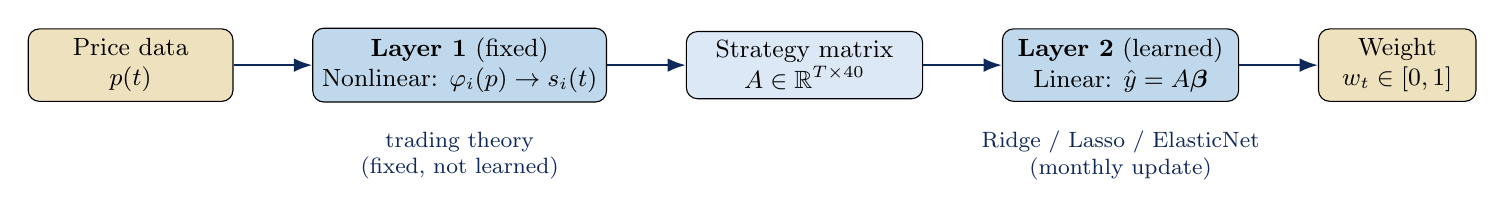
\begin{tikzpicture}[
  node distance=0.5cm and 1.0cm,
  box/.style={draw, rounded corners, minimum width=2.6cm, minimum height=0.8cm,
              align=center, font=\small},
  arrow/.style={-{Latex}, thick, color=qNavy},
]
  \node[box, fill=qGold!30] (price) {Price data\\$p(t)$};
  \node[box, right=of price, fill=qMid!25, minimum width=3.6cm] (layer1)
    {\textbf{Layer 1} (fixed)\\Nonlinear: $\varphi_i(p) \to s_i(t)$};
  \node[box, right=of layer1, fill=qLight, minimum width=3.0cm] (matA)
    {Strategy matrix\\$A \in \mathbb{R}^{T \times 40}$};
  \node[box, right=of matA, fill=qMid!25, minimum width=3.0cm] (layer2)
    {\textbf{Layer 2} (learned)\\Linear: $\hat{y} = A\boldsymbol{\beta}$};
  \node[box, right=of layer2, fill=qGold!30, minimum width=2.0cm] (weight)
    {Weight\\$w_t \in [0,1]$};

  \draw[arrow] (price)  -- (layer1);
  \draw[arrow] (layer1) -- (matA);
  \draw[arrow] (matA)   -- (layer2);
  \draw[arrow] (layer2) -- (weight);

  \node[below=0.25cm of layer1, font=\footnotesize, color=qNavy, align=center]
    {trading theory\\(fixed, not learned)};
  \node[below=0.25cm of layer2, font=\footnotesize, color=qNavy, align=center]
    {Ridge / Lasso / ElasticNet\\(monthly update)};
\end{tikzpicture}
\caption{\textbf{Two-layer prediction architecture.} Layer 1 converts raw
price data into structured strategy signals using fixed, domain-grounded
transformations. Layer 2 learns a sparse linear combination of those signals
to predict the 130-day forward return, updated monthly on a rolling one-year
window.}
\label{fig:architecture}
\end{figure}

\begin{figure}[h]
\centering
\begin{subfigure}[t]{0.48\textwidth}
  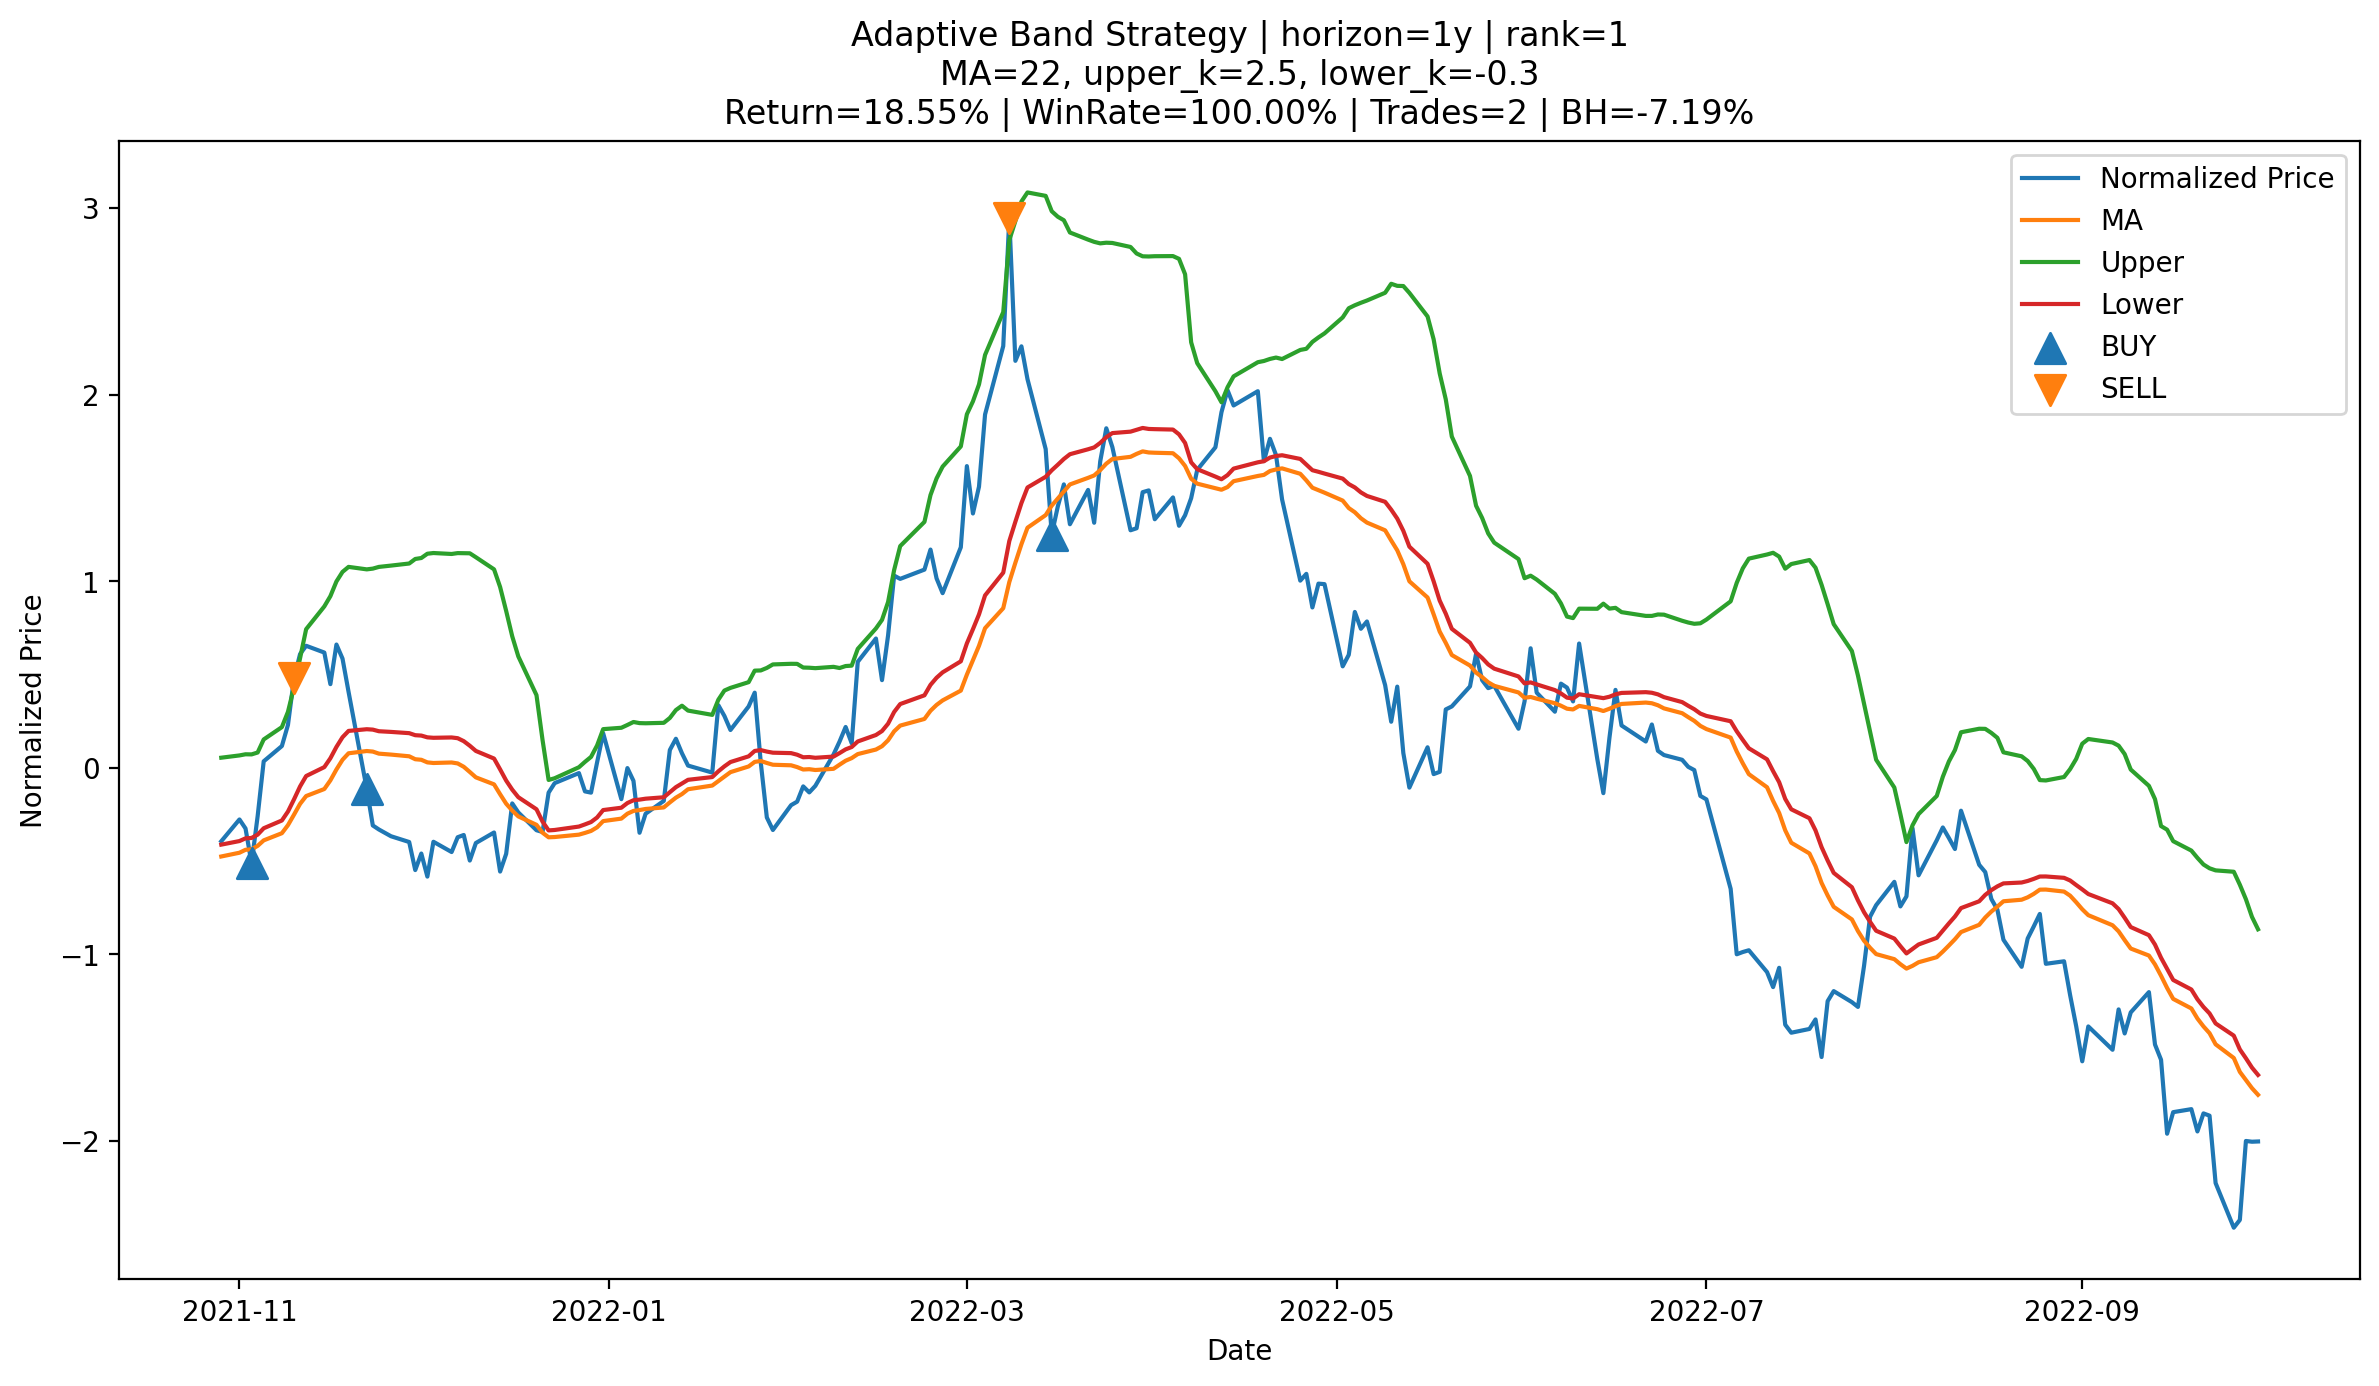
\includegraphics[width=\textwidth, height=4.5cm, keepaspectratio]
    {../../figures/adaptive_band_strategy/1y/1y_rank01_ma22_uk2.5_lk-0.3.png}
  \caption{Adaptive Band Strategy (top-ranked, 1-year window). Signal $+1$
  when price exceeds upper band, $-1$ below lower band.}
  \label{fig:strat_band}
\end{subfigure}
\hfill
\begin{subfigure}[t]{0.48\textwidth}
  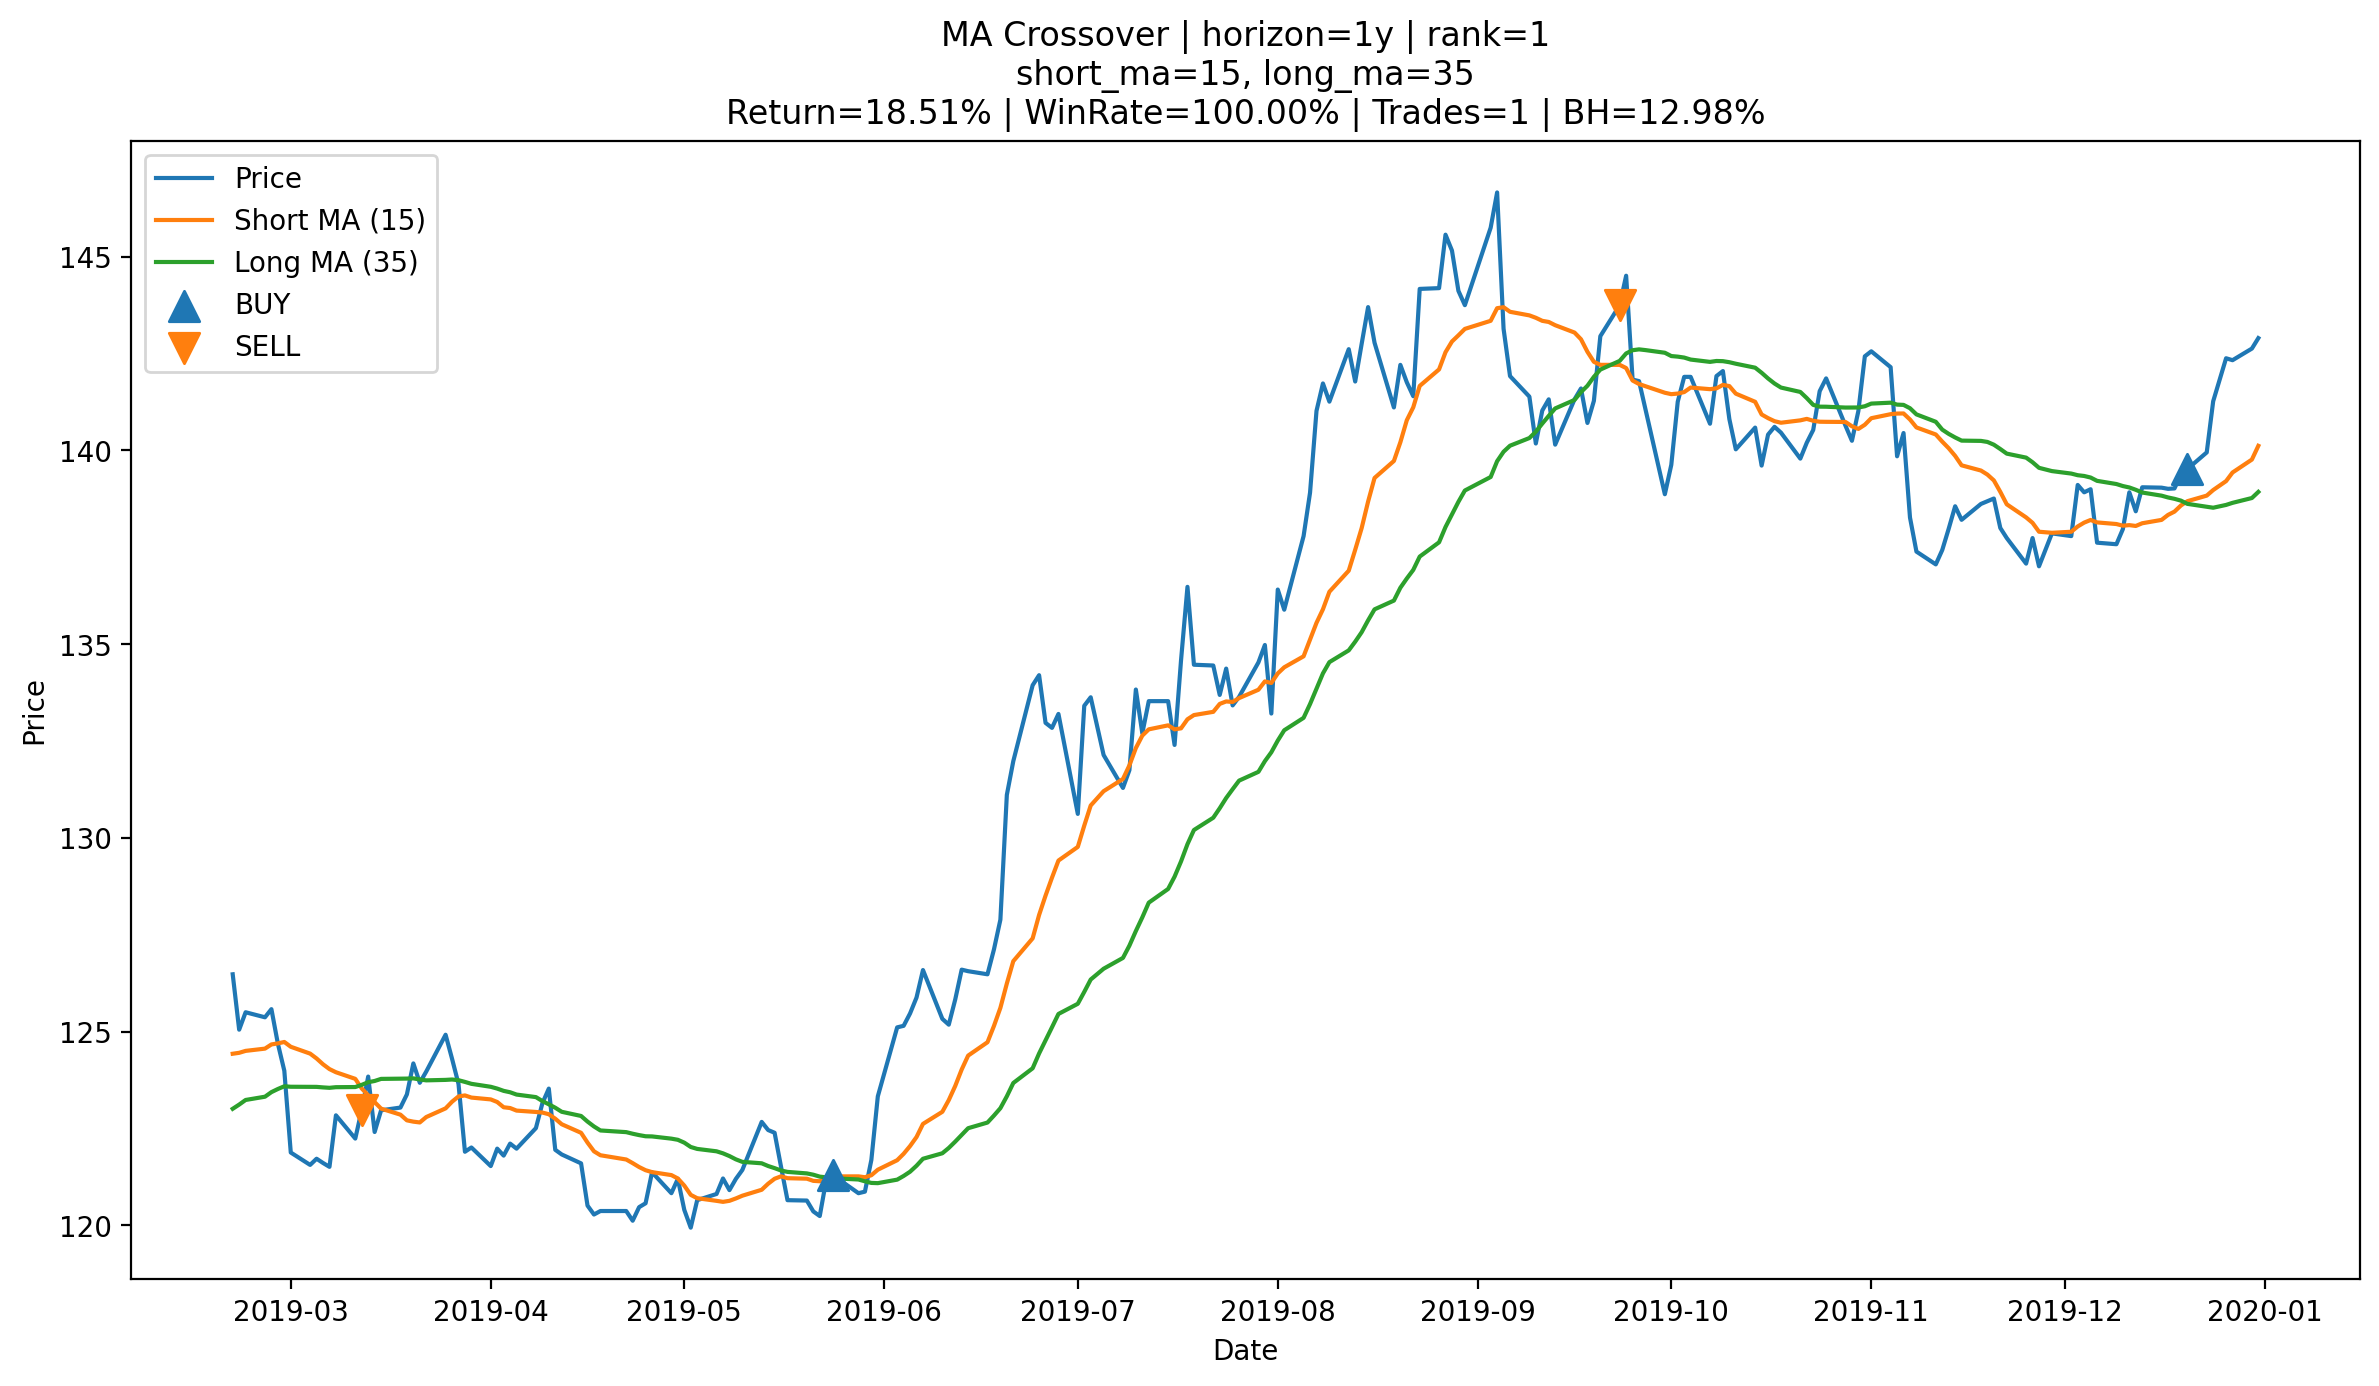
\includegraphics[width=\textwidth, height=4.5cm, keepaspectratio]
    {../../figures/ma_crossover/1y/1y_rank01_sma15_lma35.png}
  \caption{MA Crossover Strategy (top-ranked, 1-year window). Signal $+1$
  when short MA crosses above long MA, $-1$ when below.}
  \label{fig:strat_ma}
\end{subfigure}
\caption{\textbf{Example strategy signals from Layer 1.} Each plot shows
GLD price (top panel) and the continuous strategy score $s_\theta(t) \in
[-1, +1]$ (bottom panel). Different parameter choices $\theta$ produce
distinct vectors in the strategy space $\mathcal{S}$, spanning different
aspects of price dynamics. The two families shown here are among the four
used to construct the design matrix $A$.}
\label{fig:strategies}
\end{figure}

\begin{figure}[h]
\centering
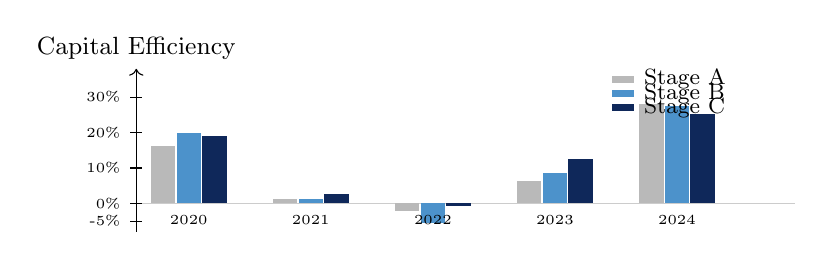
\begin{tikzpicture}[xscale=1.55, yscale=4.5]
  % Zero line + axes
  \draw[gray!40] (0.5,0) -- (5.9,0);
  \draw[->] (0.5,-0.08) -- (0.5,0.38) node[above, font=\small] {Capital Efficiency};

  % y-axis ticks
  \foreach \v/\lbl in {-0.05/-5\%,0/0\%,0.10/10\%,0.20/20\%,0.30/30\%} {
    \draw (0.45,\v) -- (0.55,\v);
    \node[left,font=\tiny] at (0.45,\v) {\lbl};
  }

  % 2020  A=16.3  B=20.0  C=19.1
  \fill[gray!55]  (0.62,0) rectangle (0.82, 0.163);
  \fill[qMid!70]  (0.83,0) rectangle (1.03, 0.200);
  \fill[qNavy]    (1.04,0) rectangle (1.24, 0.191);
  \node[below,font=\tiny] at (0.93,-0.008) {2020};

  % 2021  A=1.2  B=1.2  C=2.8
  \fill[gray!55]  (1.62,0) rectangle (1.82, 0.012);
  \fill[qMid!70]  (1.83,0) rectangle (2.03, 0.012);
  \fill[qNavy]    (2.04,0) rectangle (2.24, 0.028);
  \node[below,font=\tiny] at (1.93,-0.008) {2021};

  % 2022  A=-2.0  B=-5.5  C=-0.6
  \fill[gray!55]  (2.62,-0.020) rectangle (2.82, 0);
  \fill[qMid!70]  (2.83,-0.055) rectangle (3.03, 0);
  \fill[qNavy]    (3.04,-0.006) rectangle (3.24, 0);
  \node[below,font=\tiny] at (2.93,-0.008) {2022};

  % 2023  A=6.4  B=8.7  C=12.5
  \fill[gray!55]  (3.62,0) rectangle (3.82, 0.064);
  \fill[qMid!70]  (3.83,0) rectangle (4.03, 0.087);
  \fill[qNavy]    (4.04,0) rectangle (4.24, 0.125);
  \node[below,font=\tiny] at (3.93,-0.008) {2023};

  % 2024  A=28.1  B=27.6  C=25.2
  \fill[gray!55]  (4.62,0) rectangle (4.82, 0.281);
  \fill[qMid!70]  (4.83,0) rectangle (5.03, 0.276);
  \fill[qNavy]    (5.04,0) rectangle (5.24, 0.252);
  \node[below,font=\tiny] at (4.93,-0.008) {2024};

  % Legend
  \fill[gray!55] (4.4,0.34) rectangle (4.58,0.36);
  \node[right,font=\footnotesize] at (4.58,0.35) {Stage A};
  \fill[qMid!70] (4.4,0.30) rectangle (4.58,0.32);
  \node[right,font=\footnotesize] at (4.58,0.31) {Stage B};
  \fill[qNavy]   (4.4,0.26) rectangle (4.58,0.28);
  \node[right,font=\footnotesize] at (4.58,0.27) {Stage C};
\end{tikzpicture}
\caption{\textbf{Capital efficiency by stage and year (GLD, 2020--2024).}
Capital efficiency is defined as annual strategy return divided by average
capital exposure. Stage C (navy) achieves the highest efficiency in every
year. All three stages remain near zero or positive in the 2021 bear year
(GLD $-$6.2\%), while Stage C additionally avoids the 2022 drawdown better
than Stages A and B.}
\label{fig:stage_comparison}
\end{figure}

\begin{figure}[h]
\centering
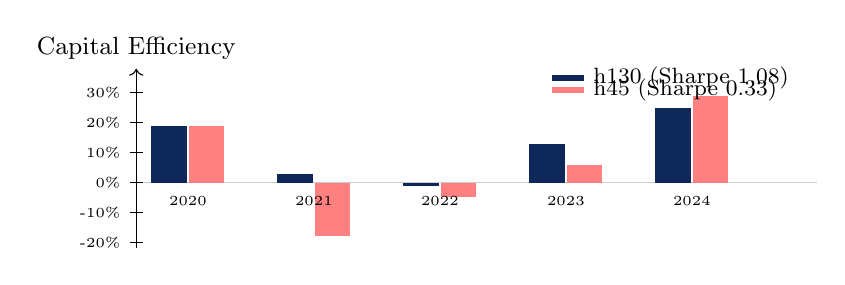
\begin{tikzpicture}[xscale=1.6, yscale=3.8]
  % Zero line + axes
  \draw[gray!40] (0.5,0) -- (5.9,0);
  \draw[->] (0.5,-0.22) -- (0.5,0.38) node[above,font=\small] {Capital Efficiency};

  % y-axis ticks
  \foreach \v/\lbl in {-0.20/-20\%,-0.10/-10\%,0/0\%,0.10/10\%,0.20/20\%,0.30/30\%} {
    \draw (0.45,\v) -- (0.55,\v);
    \node[left,font=\tiny] at (0.45,\v) {\lbl};
  }

  % 2020  h130=+19%  h45=+19%
  \fill[qNavy]  (0.62, 0) rectangle (0.90, 0.19);
  \fill[red!50] (0.92, 0) rectangle (1.20, 0.19);
  \node[below,font=\tiny] at (0.91,-0.015) {2020};

  % 2021  h130=+3%  h45=-18%
  \fill[qNavy]  (1.62, 0)     rectangle (1.90,  0.03);
  \fill[red!50] (1.92,-0.18)  rectangle (2.20,  0);
  \node[below,font=\tiny] at (1.91,-0.015) {2021};

  % 2022  h130=-1%  h45=-5%
  \fill[qNavy]  (2.62,-0.01)  rectangle (2.90, 0);
  \fill[red!50] (2.92,-0.05)  rectangle (3.20, 0);
  \node[below,font=\tiny] at (2.91,-0.015) {2022};

  % 2023  h130=+13%  h45=+6%
  \fill[qNavy]  (3.62, 0) rectangle (3.90, 0.13);
  \fill[red!50] (3.92, 0) rectangle (4.20, 0.06);
  \node[below,font=\tiny] at (3.91,-0.015) {2023};

  % 2024  h130=+25%  h45=+29%
  \fill[qNavy]  (4.62, 0) rectangle (4.90, 0.25);
  \fill[red!50] (4.92, 0) rectangle (5.20, 0.29);
  \node[below,font=\tiny] at (4.91,-0.015) {2024};

  % Legend
  \fill[qNavy]  (3.8, 0.34) rectangle (4.05, 0.36);
  \node[right,font=\footnotesize] at (4.05,0.35) {h130 (Sharpe 1.08)};
  \fill[red!50] (3.8, 0.30) rectangle (4.05, 0.32);
  \node[right,font=\footnotesize] at (4.05,0.31) {h45 (Sharpe 0.33)};
\end{tikzpicture}
\caption{\textbf{Horizon comparison: h130 vs h45 capital efficiency
(2020--2024, Stage C, top-10).} The h45 model achieves higher peak
efficiency in bull years (2024: $+$29\% vs $+$25\%) but fails
catastrophically in the 2021 bear year ($-$18\% vs $+$3\%), yielding a
Sharpe ratio of 0.33 vs 1.08. The asymmetric failure is attributed to
feature--target misalignment: Layer 1 features encode six-month dynamics
while h45 targets 45-day returns.}
\label{fig:horizon}
\end{figure}

% =============================================================================
% SUPPLEMENTAL FIGURES
% =============================================================================
\clearpage
\appendix
\section*{Supplemental Figures}

\begin{figure}[h]
\centering
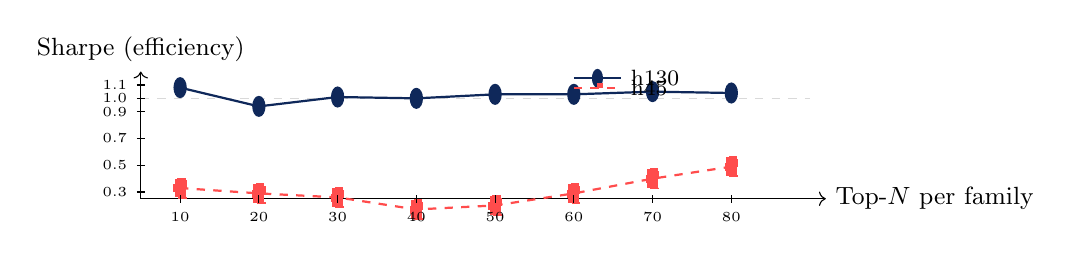
\begin{tikzpicture}[xscale=1.0, yscale=1.7]
  % axes — y range 0.25 to 1.15
  \draw[->] (0.5, 0.25) -- (9.2, 0.25) node[right, font=\small] {Top-$N$ per family};
  \draw[->] (0.5, 0.25) -- (0.5, 1.20) node[above, font=\small] {Sharpe (efficiency)};
  \draw[gray!30, dashed] (0.5, 1.0) -- (9.0, 1.0);

  % h130 line — actual data: top10=1.08, 20=0.94, 30=1.01, 40=1.00, 50=1.03, 60=1.03, 70=1.05, 80=1.04
  \draw[qNavy, thick] plot[mark=*, mark size=2pt] coordinates {
    (1,1.08)(2,0.94)(3,1.01)(4,1.00)(5,1.03)(6,1.03)(7,1.05)(8,1.04)
  };

  % h45 line — actual data: 10=0.33, 20=0.29, 30=0.26, 40=0.17, 50=0.20, 60=0.29, 70=0.40, 80=0.49
  \draw[red!70, thick, dashed] plot[mark=square*, mark size=2pt] coordinates {
    (1,0.33)(2,0.29)(3,0.26)(4,0.17)(5,0.20)(6,0.29)(7,0.40)(8,0.49)
  };

  % x-axis ticks
  \foreach \x/\n in {1/10, 2/20, 3/30, 4/40, 5/50, 6/60, 7/70, 8/80} {
    \draw (\x, 0.22) -- (\x, 0.28);
    \node[below, font=\tiny] at (\x, 0.22) {$\n$};
  }

  % y-axis ticks
  \foreach \v/\lbl in {0.3/0.3, 0.5/0.5, 0.7/0.7, 0.9/0.9, 1.0/1.0, 1.1/1.1} {
    \draw (0.45, \v) -- (0.55, \v);
    \node[left, font=\tiny] at (0.45, \v) {\lbl};
  }

  % Legend
  \draw[qNavy, thick]       (6.0, 1.15) -- (6.6, 1.15); \fill[qNavy]  (6.3,1.15) circle(2pt);
  \node[right,font=\footnotesize] at (6.6, 1.15) {h130};
  \draw[red!70,thick,dashed](6.0, 1.08) -- (6.6, 1.08); \fill[red!70] (6.3,1.08) rectangle (6.37,1.115);
  \node[right,font=\footnotesize] at (6.6, 1.08) {h45};
\end{tikzpicture}
\caption{\textbf{Supplemental Figure S1: Sharpe ratio vs top-$N$ per family
(GLD, 2020--2024).} The h130 Sharpe peaks at $N = 10$ (1.08), drops at
$N = 20$ (0.94), and partially recovers to 1.03--1.05 at $N = 50$--70,
indicating that the top-10 strategies per family are already near-optimal.
The h45 Sharpe remains consistently low across all $N$ (0.17--0.49),
confirming that horizon alignment dominates over feature count.}
\label{fig:topn}
\end{figure}

% =============================================================================
% REFERENCES
% =============================================================================
\clearpage
\bibliographystyle{plainnat}
\bibliography{references}

% =============================================================================
% REFLECTION
% =============================================================================
\clearpage
\section*{Reflection}

\textit{This section is informal and written in first person, as a personal
reflection on the research process.}

\bigskip

When I started this project, I thought I was building a trading system. By the
end, I realized I had accidentally built a framework for thinking about what
``features'' even mean in a time-series setting---and that turned out to be the
more interesting result.

The most surprising thing was the horizon alignment finding. I had assumed that
using more data (a longer horizon) would always be safer, or that shorter
horizons would at least diversify risk by capturing more cycles. The 2021 bear
year completely shattered that intuition. The short-horizon model didn't just
underperform---it catastrophically failed in exactly the year where you most
need a model to work. When I traced back why, it clicked: the features I was
feeding into the regression were calibrated by a six-month evaluation window,
and if the regression was trying to predict a 45-day outcome from six-month
features, there was a fundamental mismatch baked into the architecture. That
connection between the structure of Layer 1 and the appropriate target of
Layer 2 was not something I planned; I found it by doing the experiment and
asking ``why does this fail so badly in 2021?'' I think that's how a lot of
good research happens.

The most challenging part was keeping honest about what I was actually
measuring. Capital efficiency as a metric sounds reasonable, but I spent a lot
of time making sure the rolling tranche structure didn't introduce any
look-ahead bias---any scenario where today's decision could implicitly use
tomorrow's data. The rolling-forward validation design ended up being more
thought-intensive than the modeling itself. It's the kind of thing that's easy
to get wrong in a way that makes your results look much better than they are,
and I kept going back to double-check.

If I could do this again, I would start the multi-asset expansion much
earlier. The oracle simulation I ran at the end showed that the theoretical
upper bound for a GLD+BRK-B+QQQ system is a Sharpe of 3.02---and I'm
currently sitting at 1.08 on GLD alone with real models. That gap between the
oracle bound and what the actual model achieves is arguably the most
interesting research question in the whole project, and I only got to frame it
in the last session before the deadline.

I also learned something about my own research process: I work best when I
have a concrete, falsifiable question. The question ``does the 130-day horizon
outperform the 45-day horizon in a 2021 bear market?'' is very answerable.
``What is the best trading strategy?'' is not. Narrowing the question down to
something measurable was consistently the step that unlocked progress. I'll
take that forward into any research I do next.

\end{document}
